\documentclass{tufte-book}

\usepackage{amsmath, amsthm}
\usepackage{graphicx}
\setkeys{Gin}{width=\linewidth,totalheight=\textheight,keepaspectratio}
\graphicspath{{graphics/}}

\title{STATS 244 \\ Homework 3}
\author{Joe Seidel}
\date{\today}

\usepackage{booktabs}
\usepackage{units}
\usepackage{fancyvrb}
\fvset{fontsize=\normalsize}
\usepackage{multicol}
\usepackage{lipsum}
\usepackage{pdfpages}
\usepackage{tikz}
\usepackage{wasysym}

\newcommand{\doccmd}[1]{\texttt{\textbackslash#1}}% command name -- adds backslash automatically
\newcommand{\docopt}[1]{\ensuremath{\langle}\textrm{\textit{#1}}\ensuremath{\rangle}}% optional command argument
\newcommand{\docarg}[1]{\textrm{\textit{#1}}}% (required) command argument
\newenvironment{docspec}{\begin{quote}\noindent}{\end{quote}}% command specification environment
\newcommand{\docenv}[1]{\textsf{#1}}% environment name
\newcommand{\docpkg}[1]{\texttt{#1}}% package name
\newcommand{\doccls}[1]{\texttt{#1}}% document class name
\newcommand{\docclsopt}[1]{\texttt{#1}}% document class option name
\DeclareMathOperator{\proj}{proj}
\newcommand{\vct}{\mathbf}


\newcommand{\dprod}[2]{\langle #1, #2 \rangle}
\newcommand{\Var}{\mathrm{Var}}
\newcommand{\Cov}{\mathrm{Cov}}

\newtheoremstyle{mytheoremstyle} % name
	{\topsep}		% Space above
	{\topsep}		% Space below
	{\itshape}		% Body font
	{}			% Indent amount
	{\bfseries}	% Theorem head font
	{\textnormal{:}}	% Punctuation after theorem head
	{.5em}		% Space after theorem head
	{}			%Theorem headspec
\theoremstyle{mytheoremstyle}
\newtheorem*{thm}{Thm.}

\newtheoremstyle{mylemstyle} % name
	{\topsep}		% Space above
	{\topsep}		% Space below
	{\itshape}		% Body font
	{}			% Indent amount
	{\bfseries}	% Theorem head font
	{\textnormal{:}}	% Punctuation after theorem head
	{.5em}		% Space after theorem head
	{}			%Theorem headspec
\theoremstyle{mylemstyle}
\newtheorem*{lem}{Lem.}


\newtheoremstyle{mydefstyle} % name
	{\topsep}		% Space above
	{\topsep}		% Space below
	{\normalfont}	% Body font
	{}			% Indent amount
	{\bfseries}	% Theorem head font
	{\textnormal{:}}	% Punctuation after theorem head
	{.5em}		% Space after theorem head
	{}			%Theorem headspec
\theoremstyle{mydefstyle}
\newtheorem*{mydef}{Def.}
\newtheorem*{ex}{E.g.}

\begin{document}

\maketitle
\pagenumbering{gobble}
\newpage
\pagenumbering{arabic}

\subsection{Rice Chapter 4, Question 78}
Show that if a density is symmetric about zero, its skewness is zero.

\newthought{Skewness} can be determined using $E(X^3)$.   For example if $E(X^3)$ is zero, then skewness is zero.

Let $f_y$ be a density symmetric around zero.  Then, because of this symmetry $-f_Y = f_y$.  Which implies $E(Y^3) = E(-Y^3)$  Which means that $E(Y^3)=0$.

\subsection{Question 2}
Consider the bivariate density of $X$ and $Y$
\[f(x,y) = 4(x+y+xy)/5 \text{ for } 0< x,y <1 ,\ 0 \text{ otherwise} \]

\begin{enumerate}

\item Verify that this is a bivariate density\\
(the total volume of $\int\int f(x,y)dxdy =1$).

\begin{align*}
\int \int f(x,y)dxdy &= \int_0^1 \int_0^1 \frac{4}{5}(x+y+xy)dxdy\\
&= \int_0^1 [\frac{4}{5} (\int_0^1 x+y+xy dx)]dy\\
&= \int_0^1 [\frac{4}{5} (\int_0^1 xdx + \int_0^1ydx + \int_0^1 xydx)]dy\\
&= \int_0^1 [\frac{4}{5} (\frac{x^2}{2}\big|_0^1 + y + y(\frac{x^2}{2}\big|_0^1))]dy\\
&= \int_0^1 [\frac{4}{5} (\frac{1}{2} + 1 \frac{y}{2})]dy\\
&= \int_0^1 \frac{4}{5}(\frac{3y}{2} + \frac{1}{2})dy\\
&= \int_0^1 \frac{4}{10}(3y + 1) dy\\
&= \frac{4}{10} [\int_0^1 3ydy + \int_0^1 1 dy]\\
&= \frac{4}{10} [3(\frac{1}{2}) + 1]\\
&= \frac{4}{10} [\frac{3}{2} + 1]\\
&= 1\\
\end{align*}

\item Find the marginal density of $Y$
\marginnote{We basically found this in a step from part 1}
\begin{align*}
f_Y(y) &= \int_0^1 f_{XY}(x,y)dx\\
&= \int_0^1 \frac{4}{5}(x+y+xy)dx\\
&= \frac{4}{5} \int_0^1(x+y+xy)dx\\
&= \frac{4}{10}(3y+1)\\
\end{align*}

\item Find the conditional density of $X$ given $Y=0.5$.

\begin{align*}
f_{X\mid Y}(x \mid Y=.5) &= \frac{f(x,.5)}{f_y(.5)}\\
&= \frac{\frac{4}{5}(x + .5 +.5x)}{\frac{4}{10}(2.5)}\\
&= \frac{4}{5}(1.5x + .5)\\
\end{align*}

\item Find $E(X)$, $E(X^2)$, $\Var(X)$, $E(XY)$, $\Cov(X,Y)$.

\begin{align*}
E(X) &= \int_0^1 x f_X(x) dx\\
&= \int_0^1 x \frac{4}{10}(3x+1)dx\\
&= \frac{4}{10}[\int_0^1 3x^2+xdx]\\
&= \frac{4}{10}[\int_0^1 3x^2dx + \int_0^1xdx]\\
&= \frac{4}{10}[1 + \frac{1}{2}]\\
&= \frac{3}{5}\\
\end{align*}

\begin{align*}
E(X^2) &= \int_0^1 x^2 f_X(x)dx\\
&= \int_0^1 x^2 \frac{4}{10}(3x+1)dx\\
&= \frac{4}{10} \int_0^1 3x^3 + x^2 dx\\
&= \frac{4}{10} [\frac{3}{4}x^3\Big|_0^1 + \frac{x^3}{3}\Big|_0^1]\\
&= \frac{4}{10} (\frac{3}{4} + \frac{1}{3})\\
&= \frac{13}{30}
\end{align*}

\begin{align*}
\Var(X) &= E(X^2) - E(X)^2\\
&= \frac{13}{30} - \frac{3}{5}^2\\
&= \frac{11}{150}
\end{align*}

\begin{align*}
E(XY) &= \int_0^1 \int_0^1 xy f(x,y) dxdy\\
&= \int_0^1 \int_0^1 xy \frac{4}{5}(x+y+xy)dxdy\\
&= \int_0^1 [\frac{4}{5}\int_0^1 xy(x + y +xy)dx]dy\\
&= \int_0^1 [\frac{4}{5}y(\int_0^1(x^2 + xy + x^2y)dx]dy\\
&= \int_0^1 [\frac{4}{5}y(\frac{1}{3} + y(\frac{1}{2}) + y(\frac{1}{3})]dy\\
&= \int_0^1 \frac{4}{15}y(\frac{5y}{2}+1)dy\\
&= \frac{4}{15} \int_0^1 \frac{5y^2}{2} + y dy\\
&= \frac{4}{15}[\frac{5}{6} + \frac{1}{2}]\\
&= \frac{16}{45}\\
\end{align*}

We should note that because the marginal density of $X$ and $Y$ are symmetric(?) $E(X)=E(Y)=\frac{3}{5}$.  In anycase, we don't need to compute $E(Y)$ since the marginal densities look the same.

\begin{align*}
\Cov(X,Y) &= E(XY) - E(X)E(Y)\\
&= \frac{16}{45} - \frac{3}{5}^2\\
&= -\frac{1}{225}\\
\end{align*}

\item Find $P(0.2 \leq X \leq .5 \text{ and } .4 \leq Y \leq .8)$
\marginnote{I asked for a clarification on this question on the discussion board and no one answered!}

\begin{align*}
P(0.2 \leq X \leq .5 \text{ and } .4 \leq Y \leq .8) &= \int_{.4}^{.8} \int_{.2}^{.5} f(x,y)dxdy\\
&= \int_{.4}^{.8} \int_{.2}^{.5} \frac{4}{5}(x + y + xy)dxdy\\
&= \int_{.4}^{.8}[\frac{4}{5} \int_{.2}^{.5} x+y+xy dx]dy\\
&= \int_{.4}^{.8}[\frac{4}{5}(.405y  + .105)dy\\
&= \frac{4}{5}(.0972 + .042)\\
&= .11136\\
\end{align*}
\item Find $P(X + Y \leq 1)$
Set $y=v-x$
\begin{align*}
P(X + Y \leq 1) &= \int_0^y \int_0^xf(x,v)dxdv\\
\int_0^1 \int_0^{1-x} f(x,y)dydx\\
&= \int_0^1 \int_0^{1-x} \frac{4}{5}(x+y+xy)dydx\\
&= \int_0^1[\frac{4}{5}(\int_0^{1-x}xdy + \int_0^{1-x}ydy + x\int_0^{1-x}ydy)]dx\\
&=\int_0^1 \frac{4}{5}[-(1-x)x + \frac{1}{2}(x-1)^2+ \frac{1}{2}(x-1)^2x +]dx\\
&=\int_0^1 \frac{4}{10}(x^3 - 3x^2 + x +1)dx\\
&= \frac{4}{10}[\frac{1}{4} - 1 + \frac{1}{2} +1]\\
&= \frac{3}{10}
\end{align*}
\end{enumerate}


\subsection{Question 3, Rice 4.81 and 4.82}

\begin{enumerate}

\item Find the moment-generating function of a Bernoulli random variable, and use it to find the mean, variance, and third moment.

\newthought{A Bernoulli} random variable is one such that $f(x) = 1-p$ where $f(0) = 1-p$ and $f(1) = p$.

\begin{align*}
M(t) &= \sum e^{tx} f(x)\\
&= e^{t(0)}f(0) + e^{t(1)}f(1)\\
&= e^{t(0)}(1-p) + e^{t(1)}(p)\\
&= 1-p + e^tp\\
\end{align*}

To find the first, second and third moments, take the following derivivative of $M(t)$.
\begin{align*}
M'(t) &= pe^{t}\\
M''(t) &= pe^{t}\\
M'''(t) &= pe^{t}\\
\end{align*}

Evauluating each of these at $0$ gives us our moments, respectively.
\begin{align*}
E(X) &= p \\
E(X^2) &= p\\
E(X^3) &= p\\
\end{align*}

We also need find the variance.
\[ \Var(X) = E(X^2) - E(X)^2 = p - p^2 \]
If we let $q = 1-p$ then $\Var(X) = p(1-p) = pq$

\item Use the result of Problem 81 to find the mgf of a binomial random variable and its mean and variance.

\newthought{LET} $X_1, X_2, X_3,...,X_n$ be independently and identically distributed Bernoulli random variables with paremeter $p$.

Let $Y=X_1+X_2+X_3,...,X_n$, so $Y=\sum_{i=1}^nX_i$.  Then

\begin{align*}
M_Y(t) &= E(e^{ty})\\
&= E(e^{(tx_1 + tx_2+...+tx_n)})\\
&= E(e^{tx_1})E(e^{tx_2})...E(e^{tx_n})\\
&= M_{x_1}(t)M_{x_2}(t)...M_{x_n}(t)\\
&= (1-p + pe^t)^n
\end{align*}

Now we take the first and second derivates of $M_Y(t)$ in order to find the first and second moments.

\begin{align*}
M_Y'(t) &= \frac{d}{dt}(1-p+e^tp)^n\\
&= n(1-p+e^tp)^{n-1} \frac{d}{dt}(1-p+e^tp)\\
&= n(1-p+e^tp)^{n-1} e^{t}p\\
&= npe^t(1-p+pe^t)^{n-1}\\
\end{align*}

\begin{align*}
M_Y''(t) &= \frac{d}{dt}npe^t(1-p+pe^t)^{n-1}\\
&= np\frac{d}{dt}e^t(1-p+pe^t)^{n-1}\\
&= np[(1-p+pe^t)^{n-1} \frac{d}{dt}e^t + e^t(\frac{d}{dt}(1-p+pe^t)^{n-1})]\\
&= np[(1-p+pe^t)^{n-1}e^t + e^t(n-1)(1-p+pe^t)^{n-2}\frac{d}{dt}(1-p+pe^t)]\\
&= np[(1-p+pe^t)^{n-1}e^t + e^t(n-1)(1-p+pe^t)^{n-2}pe^t]\\
&= np[e^t(1-p+pe^t)^{n-1}+ pe^{2t}(n-1)(1-p+pe^t)^{n-2}]\\
\end{align*}

Find $E(X)$ by evauluating $M'(t)$ at zero.

\begin{align*}
E(X) &= M'(0)\\
&= npe^0 (1-p+pe^0)^{n-1}\\
&= np(1-p+p)^{n-1}\\
&= np
\end{align*}

Similarily we find $E(X^2)$.

\begin{align*}
E(X^2) &= M''(0)\\
&= np[e^0(1-p+pe^0)^{n-1}+ pe^{2(0)}(n-1)(1-p+pe^0)^{n-2}]\\
&= np[(1-p+p)^{n-1} + p(n-1)(1-p+p)^{n-2}]\\
&= np[1 + p(n-1)]\\
\end{align*}

Now the variance can be found.

\begin{align*}
\Var(X) &= E(X^2) - E(X)^2\\
&= np + n^2p^2 - np^2 - n^2p^2\\
&= np - np^2\\
&= np(1-p)\\
\end{align*}
\end{enumerate}


\subsection{Question 5 Rice 5.6}
Using moment-generating functions, show that as $\alpha \to \infty$, the gamma distribution with parameters $\alpha$ and $\lambda$, properly standardized, tends to the standard normal distribution.

\newthought{From the} Continuity Theorem, if we can show that a sequence of gamma functions converges to the moment generating function of the standard normal distribution, then the gamma function also converges to the standard normal.

Since the question mentions standardization, we'll use the MGF of the gamma function to find means and standard deviations.

First suppose we have a random variable $X_n$ with gamma distribution.
\[ f_X(x) = \frac{\lambda^{\alpha}}{\Gamma(\alpha)} x^{\alpha-1}e^{-\lambda x} \]
The moment generating function is given.

\[M(t) = (\frac{\lambda}{\lambda-t})^\alpha ,\ t < \lambda \]

\begin{align*}
M'(t) &= \alpha(\frac{\lambda}{\lambda-t})^{\alpha-1}(\frac{d}{dt}\frac{\lambda}{\lambda-t})\\
&= \alpha(\frac{\lambda}{\lambda-t})^{\alpha-1} \lambda(\frac{d}{dt}\frac{1}{\lambda-t})\\
&= \alpha \lambda(\frac{\lambda}{\lambda-t})^{\alpha-1} (\lambda-t)^{-2}\\
&= \alpha \lambda^{a}(\lambda-t)^{-a-1}\\
\end{align*}

\begin{align*}
M''(t) &=\frac{d}{dt} \alpha \lambda^{a}(\lambda-t)^{-a-1}\\
&= \alpha \lambda^{a} \frac{d}{dt}(\lambda-t)^{-a-1}\\
&=  \alpha \lambda^{\alpha} (\alpha+1)(\lambda-t)^{-\alpha-2}\\
\end{align*}

Now we have enough to find the mean and variance of the Gamma distribution.

\begin{align*}
E(X) &= \frac{\alpha}{\lambda}\\
E(X^2) &= \frac{\alpha(\alpha+1)}{\lambda^2}\\
\end{align*}
So
\[ \Var(X) = \frac{\alpha}{\lambda^2} \]

Now we have enough to standarize $X$.  We will let $Z$ be the standarized version of our $X$.

\begin{align*}
f_{Z_n}(x) &= \frac{X_n - E(X)}{\sqrt{\Var(X)}}\\
&= \frac{X_n - \frac{\alpha}{\lambda}}{\sqrt{\frac{\alpha}{\lambda^2}}}\\
&= \frac{X_n \lambda}{\sqrt{\alpha}} - \sqrt{\alpha}\\
\end{align*}

It follows from Property C of section 4.5 that

\begin{align*}
M_{Z_n} &= E(e^{tX_n})\\
&= e^{-t\sqrt{\alpha_n}} M_{X_n}(\frac{\lambda }{\sqrt{\alpha_n}})\\
&= e^{-t\sqrt{\alpha_n}} (\frac{\lambda}{\lambda-\frac{\lambda t}{\sqrt{\alpha_n}}})^\alpha\\
&= e^{-t\sqrt{\alpha_n}}  (1-\frac{t}{\sqrt{\alpha_n}})^{-\alpha}\\
\end{align*}

Taking the limit of this function as $\alpha$ approaches infinity.

\[ \lim_{\alpha \to \infty}M_z(t) = e^{\frac{t^2}{2}} \]

Which is the desired result.


\subsection{Question 5}
Suppose that a Bayesian statistican has a Beta(2,1) prior distribution on the cure rate $\theta$ (= Probability of cure) for an experimental drug.  The drug is tried (independently) on three subjects and $X$ are cured.  Compute $P(\theta \leq 0.2 \mid X =k)$ and $E(\theta \mid X=k)$ for $k=0,1,2,3$.

\newthought{The prior} distribution turns out to be

\[ f_\Theta(\theta) = 2\theta  \text{ for } 0 \leq \theta \leq 1\]

We observe $X$ Bernoulli random variables with with conditional probabilty $\theta$ which forms a binomial distribution given

\[f_{X\mid \Theta}(x \mid \theta) = \binom{n}{x}\theta^x(1-\theta)^{n-x} \]

To find $(P \theta \mid X=k$) for $k=0,1,2,3$ first consider.

\begin{align*}
f(\theta \mid x) &= \frac{f(x \mid \theta) f_\Theta(\theta)}{\int_0^1 f(x \mid \theta) f_\Theta(\theta)dy}\\
&= \frac{\binom{n}{x}\theta^x(1-\theta)^{n-x} 2\theta}{\int_0^1 \binom{n}{x}\theta^x(1-\theta)^{n-x} 2\theta}\\
&= \frac{\theta^x(1-\theta)^{n-x} \theta}{\int_0^1 \theta^x(1-\theta)^{n-x} \theta}\\
&=\frac{\theta^{x+1}(1-\theta)^{n-x}}{\int_0^1 \theta^{x+1}(1-\theta)^{n-x}}
\end{align*}

Furthmore,
\[ f(\theta \leq 0.2 \mid k) = \frac{\int_0^{.2}\theta^{k+1}(1-\theta)^{n-k}}{\int_0^1 \theta^{k+1}(1-\theta)^{n-k}}. \]

Which we can use for $k=0,1,2,3$ and observing $n=4$.
For $k=0$
\begin{align*}
f(\theta \leq 0.2 \mid 0) &= \frac{\int_0^{.2}\theta^{0+1}(1-\theta)^{3-0}}{\int_0^1 \theta^{0+1}(1-\theta)^{3-0}}\\
&= \frac{.0131}{.05}\\
&= .26
\end{align*}

For $k=1$
\begin{align*}
f(\theta \leq 0.2 \mid 0) &= \frac{\int_0^{.2}\theta^{1+1}(1-\theta)^{3-1}}{\int_0^1 \theta^{1+1}(1-\theta)^{3-1}}\\
&= \frac{.0019}{.03\bar{3}}\\
&= .058
\end{align*}

For $k=2$
\begin{align*}
f(\theta \leq 0.2 \mid 0) &= \frac{\int_0^{.2}\theta^{2+1}(1-\theta)^{3-2}}{\int_0^1 \theta^{2+1}(1-\theta)^{3-2}}\\
&= \frac{3.36*10^{-4}}{.05}\\
&= .00672
\end{align*}

For $k=3$
\begin{align*}
f(\theta \leq 0.2 \mid 0) &= \frac{\int_0^{.2}\theta^{3+1}(1-\theta)^{3-3}}{\int_0^1 \theta^{3+1}(1-\theta)^{3-3}}\\
&= \frac{6.4*10^{-5}}{.2}\\
&= 3.2*10^{-4}
\end{align*}

Since before we observed any data

\[ E(\theta) = \frac{\alpha}{\alpha+\beta} \]

and our postier distribution is also a beta distribution

\[ E(\theta \mid X=k) = \frac{\alpha + k}{\alpha+\beta + n}. \]

For $k=0$
\begin{align*}
E(\theta \mid X=0) &= \frac{\alpha + 0}{\alpha+\beta + 3}\\
&= 0.4
\end{align*}

For $k=1$
\begin{align*}
E(\theta \mid X=1) &= \frac{\alpha + 1}{\alpha+\beta + 3}\\
&= 0.5
\end{align*}

For $k=2$
\begin{align*}
E(\theta \mid X=2) &= \frac{\alpha + 2}{\alpha+\beta + 3}\\
&= \frac{2}{3}
\end{align*}

For $k=3$
\begin{align*}
E(\theta \mid X=3) &= \frac{\alpha + 3}{\alpha+\beta + 3}\\
&= \frac{5}{6}
\end{align*}


\subsection{Question 6}
Laplace's rule of succession.  What is the \textit{a posteriori} expectation of the probability that the sun will rise tomorrow given that it has risen $n$ days in a row and that before those $n$ days began we had an \textit{a priori} uniform distribution for the probability that the sun would rise? [This is a classical problem.]

\newthought{The} \textit{a priori} probability that sun will rise is
\[f_\Theta(\theta) = 1 , \ 0\leq \theta \leq 1 \text{ and } 0 \text{ otherwise.}\]

The probabilty of $X$ conditional on $\theta$ is

\[ p(X \mid \Theta) = \binom{n}{x}\theta^x(1-\theta)^{n-x}. \]

We observe $n$ events with $X=n$ occurances of the sun rising.  So

\[ f(\theta \mid X=n) \propto \binom{n}{n} y^n (1-\theta)^0 * 1\]

Which is a Beta density with $\alpha=n+1$ and $\beta=1$.  Therefore the \textit{a posteriori} expectation of the probability that the sun will rise is

\begin{align*}
E(\theta \mid X=n) &= \frac{\alpha + x}{\alpha + \beta + n}\\
&= \frac{n+1 + n}{n + 1 + 1 +n}\\
&= \frac{2n+1}{2n+2}.\\
\end{align*}


\subsection{Question 7, Rice 8.63 and 8.64}

\begin{enumerate}

\item Suppose that $100$ item are sampled from a manufacturing process and $3$ are found to be defective.  A beta prior is used for the unknown proportion $\theta$ of defective items.  Consider two cases: (1) $a=b=1$, and $a=0.5$ and $b=5$.  Plot the two posterior distributions and compare them.  Find the two posterior means and compare them.  Explain the differenes.

\newthought{Recalling} that

\[f(\theta \mid x) \propto f(x \mid \theta) f(\theta) \]

and that a Beta distribution with $a=b=1$ is a uniform distribution.  We have

\[f(\theta \mid x) \propto \theta^{3}(1-\theta)^{97} * 1. \]

A Beta distribution with $\alpha=4$ and $\beta=98$.  Knowing this we can compute the posterior mean.

\begin{align*}
E(\theta \mid X=3) &= \frac{\alpha}{\alpha + \beta}\\
&= \frac{3}{102}
&= .039
\end{align*}

For case (2) we are given $\alpha=.5$ and $\beta=5$.  So our prior distribution for $\Theta$ is given

\[ f_\Theta(\theta) = \frac{\Gamma(.5+5)}{\Gamma(.5)\Gamma(5)} \theta^{-.5} (1-\theta)^4 \]

So

\[ f(\theta \mid X=3) \propto \theta^3 (1-\theta)^{97} * \frac{\Gamma(.5+5)}{\Gamma(.5)\Gamma(5)} \theta^{-.5} (1-\theta)^4 \]

Which simplifies to another beta distribution with $\alpha=3.5$ and $\beta=102$.

So once more we can computer the posterior mean.

\begin{align*}
E(\theta \mid X=3) &= \frac{\alpha}{\alpha + \beta}\\
&= \frac{3.5}{102 + 3.5}\\
&= .0333
\end{align*}
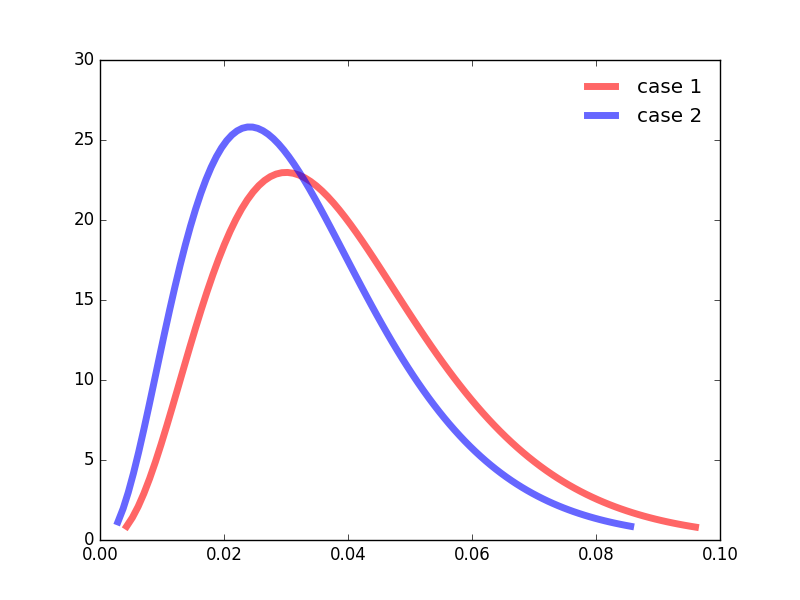
\includegraphics{figure_1}

\newthought{Compairing} the means and the plotted distributions we see that with a slighly larger $\alpha$ from case 1 that our observed values result in a larger posterier mean.  Additionally, the distribution does not rise or fall as sharply as case 2.  This helps visualize the importance of choosing the correct prior.

\item This is a continuation of the previous problem.  Let $X=0$ or $1$ according to whether an item is defective.  For each choice of the prior, what is the marginal distribution of $X$ before the sample is taken?  What are the marginal distributions after the sample is taken?

\newthought{In general}, the marginal distribution of $X$ before the sample is taken is

\[f_X(x) = \int f_{X\mid \Theta}(x \mid \theta) f_{\Theta}(\theta)d\theta. \]

In the context of this problem it can be written

\begin{align*}
f_X(x) &= \int_0^1 \binom{n}{x}\theta^x(1-\theta)^{n-x} \frac{\Gamma(\alpha + \beta)}{\Gamma(\alpha)\Gamma(\beta)} \theta^{\alpha-1}(1-\theta)^{\beta-1} d\theta\\
&= \binom{n}{x}\frac{\Gamma(\alpha + \beta)}{\Gamma(\alpha)\Gamma(\beta)}\int_0^1 \theta^x(1-\theta)^{n-x}\theta^{\alpha-1}(1-\theta)^{\beta-1} d\theta\\
&=\binom{n}{x}\frac{\Gamma(\alpha + \beta)}{\Gamma(\alpha)\Gamma(\beta)}\int_0^1 \theta^{x+\alpha-1}(1-\theta)^{n-x+\beta-1}d\theta\\
\end{align*}

Pluggin in values $\alpha$ and $\beta$ for each case give the marginal distribution before sampling.

For $\alpha=\beta=1$
\begin{align*}
f_X(x) &= \binom{n}{x}\frac{\Gamma(1 + 1)}{\Gamma(1)\Gamma(1)}\int_0^1 \theta^{x+1-1}(1-\theta)^{n-x+1-1}d\theta\\
&=\binom{n}{x}(1)\int_0^1 \theta^{x} (1-\theta)^{n-x}d\theta\\
&=\binom{n}{x}\frac{\Gamma(1+n-x)\Gamma(1+x)}{\Gamma(2+n)}\\
\end{align*}

For $\alpha=0.5$ and $\beta=5$
\begin{align*}
f_X(x) &= \binom{n}{x}\frac{\Gamma(0.5 + 5)}{\Gamma(0.5)\Gamma(5)}\int_0^1 \theta^{x+0.5-1}(1-\theta)^{n-x+5-1}d\theta\\
&=\binom{n}{x}\frac{\Gamma(5.5)}{\Gamma(0.5)\Gamma(5)}\int_0^1 \theta^{x-.5} (1-\theta)^{n-x+4}d\theta\\
&=\binom{n}{x}\frac{315}{256}\frac{\Gamma(1+n-x+4)\Gamma(1+x-0.5)}{\Gamma(1+x-.5+1+n-x+4)}\\
&=\binom{n}{x}\frac{315}{256}\frac{\Gamma(n-x+5)\Gamma(x+0.5)}{\Gamma(x+n-x+5.5)}\\
\end{align*}

\newthought{After} the sample is taken. We should first consider that, in general

\[ f_{\Theta \mid X}(\theta \mid x) = \frac{f_{X \mid \Theta}(x \mid \theta)f_\theta(\theta)}{f_{X}(x)}. \]

From this we have
\begin{align*}
f_X(x) &= \frac{f_{X \mid \Theta}(x \mid \theta)f_\Theta(\theta)}{f_{\Theta \mid X}(\theta \mid x)}\\
&= \frac{\binom{n}{x} \frac{\Gamma(\alpha+\beta)}{\Gamma(\alpha)\Gamma(\beta)}\theta^{x+\alpha-1}(1-\theta)^{n-x+\beta-1}}{ \frac{\Gamma(3+\alpha+100-3+\beta)}{\Gamma(3+\alpha)\Gamma(100-3+\beta)}\theta^{3+\alpha-1}(1-\theta)^{100-3+\beta-1}}\\
\end{align*}

Using this formula we can find the posterior distributions plugging values for each case.

For $\alpha=\beta=1$
\begin{align*}
f_X(x)&= \frac{\binom{n}{x} \frac{\Gamma(1+1)}{\Gamma(1)\Gamma(1)}\theta^{x+1-1}(1-\theta)^{n-x+1-1}}{ \frac{\Gamma(3+1+100-3+1)}{\Gamma(3+1)\Gamma(100-3+1)}\theta^{3+1-1}(1-\theta)^{100-3+1-1}}\\
&=\frac{\binom{n}{x} \frac{\Gamma(2)}{\Gamma(1)\Gamma(1)}\theta^{x}(1-\theta)^{n-x}}{ \frac{\Gamma(102)}{\Gamma(4)\Gamma(98)}\theta^{3}(1-\theta)^{97}}\\
&=\frac{\binom{n}{x}(1)\theta^{x-3}(1-\theta)^{n-x-97}}{ \frac{\Gamma(102)}{\Gamma(4)\Gamma(98)}}\\
&= \binom{n}{x}\frac{\Gamma(4)\Gamma(98)}{\Gamma(102)}\theta^{x-3}(1-\theta)^{n-x-97}\\
&=\binom{n}{x}\binom{96}{3}(95)\theta^{x-3}(1-\theta)^{n-x-97}\\
\end{align*}

For $\alpha=0.5$ and $\beta=5$.
\begin{align*}
f_X(x) &= \frac{\binom{n}{x} \frac{\Gamma(5.5)}{\Gamma(0.5)\Gamma(5)}\theta^{x-0.5}(1-\theta)^{n-x+4}}{ \frac{\Gamma(105.5)}{\Gamma(3.5)\Gamma(102)}\theta^{2.5}(1-\theta)^{101}}\\
 &= \frac{\binom{n}{x} \frac{\Gamma(5.5)}{\Gamma(0.5)\Gamma(5)}\theta^{x-3}(1-\theta)^{n-x-97}}{ \frac{\Gamma(105.5)}{\Gamma(3.5)\Gamma(102)}}\\
&=\binom{n}{x}\frac{\Gamma(5.5)}{\Gamma(0.5)\Gamma(5)}\frac{\Gamma(3.5)\Gamma(102)}{\Gamma(105.)}\theta^{x-3}(1-\theta)^{n-x-97}\\
\end{align*}
\end{enumerate}

\end{document}

\grid
